\documentclass{article}

% Official NeurIPS 2026 main-track submission style.
% Do not pass final or preprint options for anonymous submission.
\usepackage{neurips_2026}

\usepackage[utf8]{inputenc}
\usepackage[T1]{fontenc}
\usepackage{amsmath,amssymb,amsthm,mathtools}
\usepackage{graphicx}
\usepackage{booktabs}
\usepackage{algorithm}
\usepackage{algpseudocode}
\usepackage{microtype}
\usepackage{url}
\usepackage{xcolor}
\usepackage{hyperref}
\usepackage{cleveref}

\newtheorem{theorem}{Theorem}
\newtheorem{lemma}{Lemma}
\newtheorem{proposition}{Proposition}
\newtheorem{corollary}{Corollary}
\newtheorem{definition}{Definition}
\newtheorem{assumption}{Assumption}
\newtheorem{remark}{Remark}

\newcommand{\R}{\mathbb{R}}
\newcommand{\T}{\mathbb{T}}
\newcommand{\W}{\mathcal{W}}
\newcommand{\eps}{\varepsilon}
\newcommand{\Div}{\operatorname{div}}
\newcommand{\norm}[1]{\left\lVert #1 \right\rVert}

\title{A Fixed-Point Reduction for Extending GAN-Compatible Mean Field Game Solvers\\
with Weakly Non-Separable Hamiltonians}

\author{Anonymous Authors}

\begin{document}

\maketitle

\begin{abstract}
GAN-based solvers for mean field games (MFGs) provide a distributional approach
to learning population equilibria, but existing formulations largely rely on
separable Hamiltonians.  This restriction excludes models in which the density
interacts directly with momentum or control variables, including traffic-flow and
congestion-type MFGs.  We propose an outer fixed-point reduction that extends
GAN-compatible MFG solvers to weakly non-separable Hamiltonians of the form
\(H(x,\rho,p)=H_0(x,p)-f_0(x,\rho)+\eps R(x,\rho,p)\).  The method freezes the
density inside the non-separable residual, so that each outer iteration reduces
to a separable MFG subproblem that can be solved using existing adversarial inner
solvers.  Under Lasry--Lions monotonicity, strong convexity of the base
Hamiltonian, and boundedness assumptions on the density and momentum variables, we prove
that the exact outer map is an \(L^2\) contraction under an explicit
weak-coupling condition.  This yields convergence of the proposed outer scheme;
in the density-only subcase, the rate reduces to \(\eps L_R/\lambda\), and this
threshold is sharp for a linearized ergodic model on the torus.  Numerical
experiments validate the predicted outer-map phase transitions beyond the
separable setting.
\end{abstract}

\section{Introduction}

Learning equilibria in large interacting populations is a central challenge in
multi-agent machine learning.  Mean field games (MFGs) provide a continuum
limit in which population behavior is described by a backward
Hamilton--Jacobi--Bellman equation coupled to a forward Fokker--Planck equation
\citep{lasry2007mean,huang2006large}:
\begin{align}
  -\partial_t \varphi-\nu\Delta\varphi+H(x,\rho,\nabla\varphi)&=0,
  \label{eq:hjb}\\
  \partial_t\rho-\nu\Delta\rho-\Div\!\bigl(\rho\nabla_pH(x,\rho,\nabla\varphi)\bigr)&=0.
  \label{eq:fp}
\end{align}
Recent GAN-based MFG solvers exploit this structure to learn population
densities distributionally rather than on a fixed grid.  When
\(H(x,\rho,p)=H_0(x,p)-f_0(x,\rho)\), the system admits a variational structure
connected to Wasserstein GANs, enabling adversarial solvers such as APAC-Net and
MFGAN \citep{goodfellow2014generative,arjovsky2017wasserstein,
cao2021connecting,lin2021apac,ruthotto2020machine}.  The separability
assumption, however, excludes important models where density and momentum are
coupled directly, including traffic-flow MFGs \citep{huang2019mfg}.

We study a restricted non-separable regime in which the GAN-compatible
structure can still be used.  The key step is to freeze the density appearing
in the non-separable part; with that density fixed, the remaining subproblem is
separable in the sense required by existing GAN-based MFG solvers.  The
analysis then splits into an outer fixed-point map, which handles the
non-separable coupling, and an inner separable solver, which may be implemented
by any GAN-based MFG method.  The resulting contribution is a reduction theorem
that identifies when separable adversarial MFG solvers can be used inside a
provably contractive outer loop.

\paragraph{GAN compatibility.}
By GAN-compatible, we mean that after freezing the residual density, each outer
step becomes a separable MFG subproblem admitting the variational/adversarial
formulation used by existing GAN-based MFG solvers.  The outer theorem is
agnostic to the specific inner implementation; in the experiments below we
isolate this outer map rather than train a stochastic adversarial model.

Several alternatives address parts of this gap.  Physics-informed MFG solvers
such as MFDGM handle non-separable Hamiltonians by minimizing PDE residuals
directly, but their guarantees are not distributional contraction rates
\citep{sirignano2018dgm,raissi2019physics,assouline2023deep}.  Classical
finite-difference and policy-iteration schemes provide useful low-dimensional
reference solvers, but do not provide a GAN-compatible distributional learning
pipeline \citep{achdou2010mean,lavigne2023policy,hu2024recent}.  Our
contribution is an outer contraction principle for turning a weak
non-separable MFG into a sequence of separable subproblems.

\paragraph{Contributions.}
We make five contributions.  First, we identify a weakly non-separable class of
MFG Hamiltonians that goes beyond the separable setting used by existing
GAN-based solvers.  Second, we formulate a fixed-point outer iteration that
reduces each step to a separable MFG subproblem solvable by GAN-based inner
methods.  Third, we prove an explicit \(L^2\) contraction theorem for the exact
outer map and derive Wasserstein convergence as a corollary.  Fourth, we show
sharpness of the weak-coupling threshold in a linearized ergodic family.  Fifth,
we validate the predicted phase transition numerically, including a
traffic-flow family that motivates density--momentum coupling.

\begin{table}[t]
\centering
\begin{tabular}{lccc}
\toprule
Method family & Non-separable \(H\) & Distributional density & Explicit rate \\
\midrule
GAN-based MFG solvers & No & Yes & No / implicit \\
MFDGM / PINN residual solvers & Yes & No & No \\
Finite-difference / policy iteration & Yes & No & Problem dependent \\
This work & Weakly & Compatible with inner solvers & Exact outer map \\
\bottomrule
\end{tabular}
\caption{Positioning.  The proposed contribution is an outer contraction
framework: it keeps the separable GAN-compatible inner problem while controlling
weak non-separable residual coupling.}
\label{tab:positioning}
\end{table}

\paragraph{Scope.}
The guarantee is conditional on the quality of the separable inner solve.  It
does not prove convergence of stochastic neural-network training.  Instead, it
proves that if the inner problem is solved exactly, or up to a controlled
error, then the non-separable outer iteration contracts.  This separation is
useful because optimization guarantees for the inner GAN solver can be improved
independently of the outer fixed-point analysis.

\section{Weakly Non-Separable Hamiltonians}

\begin{definition}
A Hamiltonian is weakly non-separable with coupling strength \(\eps\geq0\) if
\begin{equation}
  H(x,\rho,p)=H_0(x,p)-f_0(x,\rho)+\eps R(x,\rho,p),
  \label{eq:decomp_neurips}
\end{equation}
where \(H_0\) is convex in \(p\), \(f_0\) is monotone in \(\rho\), and
\(R\) is the residual density--momentum coupling.
\end{definition}

The example motivating the paper is the one-parameter traffic-flow family
\begin{equation}
  H_\eps(\rho,p)=\frac12 p^2-p+\eps \rho p,
  \label{eq:traffic_family}
\end{equation}
whose case \(\eps=1\) corresponds to the common normalization
\(\frac12 p^2-(1-\rho)p\).  For fixed \(\bar\rho\), the effective Hamiltonian
\(H_0(p)+\eps R(\bar\rho,p)\) no longer depends on the unknown density and is
therefore a separable MFG subproblem.

\section{Fixed-Point Reduction}

Let \(\bar\rho\) denote the density frozen from the previous outer step.  Define
\[
  H^{\bar\rho}(x,p)=H_0(x,p)+\eps R(x,\bar\rho(x,t),p).
\]
The outer fixed-point map \(\mathcal{T}\) sends \(\bar\rho\) to the density
\(\rho\) obtained by solving the separable MFG with Hamiltonian
\(H^{\bar\rho}\) and interaction \(f_0\).

\begin{algorithm}[t]
\caption{Fixed-point wrapper for GAN-compatible MFG solvers}
\label{alg:neurips}
\begin{algorithmic}[1]
\Require decomposition \(H=H_0-f_0+\eps R\), initial density \(\rho_0\),
terminal cost \(g\), outer steps \(K\), inner steps \(N\)
\State initialize \(\rho^0\gets \rho_0\)
\For{\(k=0,\ldots,K-1\)}
  \State form \(H^k(x,p)=H_0(x,p)+\eps R(x,\rho^k(x,t),p)\)
  \State solve the separable MFG with Hamiltonian \(H^k\) using a GAN-based
  inner solver, e.g. APAC-Net:
  \[
    (\varphi^{k+1},\rho^{k+1})\gets \textsc{GAN-MFG}(H^k,f_0,g,\rho_0,N)
  \]
\EndFor
\State \Return \((\varphi^K,\rho^K)\)
\end{algorithmic}
\end{algorithm}

When the inner solver is approximate, the outer error does not disappear but is
controlled by the usual perturbed fixed-point bound.  If
\(\norm{\rho_N^{k+1}-\mathcal{T}(\rho_N^k)}_{L^2}\leq\delta_N\), then
\[
  \norm{\rho_N^k-\rho^\star}_{L^2}
  \leq \kappa_\eps^k\norm{\rho^0-\rho^\star}_{L^2}
  +\frac{\delta_N}{1-\kappa_\eps}.
\]
Here \(\kappa_\eps\) denotes the exact outer-map contraction factor defined in
\Cref{thm:l2_contraction_neurips}.
Thus the outer theory converts inner-solver accuracy into an explicit bias
floor.  The proof is in the appendix.

\section{Convergence of the Exact Outer Map}

We state the theorem for exact inner solves.  Approximation error from finite
inner training appears additively in the usual perturbed-contraction bound.

\begin{assumption}
\label{ass:neurips}
The following hold for all frozen densities considered by the iteration.
\begin{enumerate}
\item Each frozen separable subproblem has a unique solution
\((\varphi_{\bar\rho},\rho_{\bar\rho})\) in the admissible class, so
\(\mathcal{T}(\bar\rho)=\rho_{\bar\rho}\) is well defined.
\item \(H_0\) is \(c_0\)-strongly convex in \(p\).
\item \(f_0\) is \(\lambda\)-strongly monotone:
\[
  \int_\Omega (f_0(x,\rho_1)-f_0(x,\rho_2))(\rho_1-\rho_2)\,dx
  \geq \lambda\norm{\rho_1-\rho_2}_{L^2}^2 .
\]
\item Densities satisfy \(0<\rho_{\min}\leq \rho\leq\rho_{\max}\).
\item Momentum is bounded: \(\norm{\nabla\varphi_{\bar\rho}}_{L^\infty}\leq u_{\max}\).
\item On \(|p|\leq u_{\max}\), \(R\) is \(L_R\)-Lipschitz in \(\rho\), is
smooth in \(p\), and satisfies
\(|\nabla_p R|+|\nabla^2_{pp}R|\leq L_{R,p}\).  In addition,
\(\nabla_pR\) is \(L_{p\rho}\)-Lipschitz in the frozen density:
\[
  |\nabla_pR(x,\rho_1,p)-\nabla_pR(x,\rho_2,p)|
  \leq L_{p\rho}|\rho_1-\rho_2|.
\]
The \(p\)-variation is dominated by strong convexity:
\[
  3\eps L_{R,p}\rho_{\max}<c_0\rho_{\min},
\]
where the factor \(3\) is a conservative constant from the stability estimate.
\end{enumerate}
\end{assumption}

\paragraph{Examples covered by the assumptions.}
The assumptions hold for regularized MFGs on the torus with quadratic
\(H_0(p)=|p|^2/2\), linear monotone coupling \(f_0(\rho)=\lambda\rho\), and
bounded smooth residuals such as \(R(\rho,p)=a(\rho)b(p)\) on invariant sets
where \(0<\rho_{\min}\leq\rho\leq\rho_{\max}\) and \(|p|\leq u_{\max}\).  The
density-only residual \(R(\rho,p)=L_R\rho\) has \(L_{R,p}=0\), so the
momentum-domination condition is automatic and the threshold reduces to
\(\eps L_R<\lambda\).  The bilinear traffic residual \(R(\rho,p)=\rho p\)
satisfies the assumptions on bounded density--momentum sets when
\(3\eps\rho_{\max}<c_0\rho_{\min}\), with \(L_{p\rho}=1\); our traffic
experiment studies the corresponding linearized rate around the uniform
no-drift equilibrium.

\begin{theorem}[Outer contraction]
\label{thm:l2_contraction_neurips}
Under \Cref{ass:neurips}, define
\[
  \alpha_\eps=c_0\rho_{\min}-3\eps L_{R,p}\rho_{\max}>0,\qquad
  B_\eps=\frac{\eps^2L_{p\rho}^2\rho_{\max}^2}{4\alpha_\eps},
\]
and
\[
  \kappa_\eps=
  \frac{\eps L_R+\sqrt{\eps^2L_R^2+4\lambda B_\eps}}{2\lambda}.
\]
If \(\kappa_\eps<1\), then the exact
outer map \(\mathcal{T}\) is a contraction:
\[
  \norm{\mathcal{T}(\bar\rho_1)-\mathcal{T}(\bar\rho_2)}_{L^2((0,T)\times\Omega)}
  \leq
  \kappa_\eps\norm{\bar\rho_1-\bar\rho_2}_{L^2((0,T)\times\Omega)} .
\]
Consequently, the exact outer iteration satisfies
\[
  \norm{\rho^k-\rho^\star}_{L^2}
  \leq
  \kappa_\eps^k\norm{\rho^0-\rho^\star}_{L^2}.
\]
\end{theorem}

\begin{proof}[Proof sketch]
Compare two separable subproblems with frozen densities \(\bar\rho_1\) and
\(\bar\rho_2\).  Let \(\delta\rho=\rho_1-\rho_2\),
\(\delta\bar\rho=\bar\rho_1-\bar\rho_2\), and
\(\delta p=\nabla\varphi_1-\nabla\varphi_2\).  The Lasry--Lions duality identity
for \(\frac{d}{dt}\int\delta\varphi\,\delta\rho\) gives
\[
  \lambda\norm{\delta\rho}_{L^2}^2
  \leq
  \eps L_R\norm{\delta\bar\rho}_{L^2}\norm{\delta\rho}_{L^2}
  + B_\eps\norm{\delta\bar\rho}_{L^2}^2 .
\]
Solving this quadratic inequality in
\(\norm{\delta\rho}_{L^2}/\norm{\delta\bar\rho}_{L^2}\) yields
\(\kappa_\eps\).  Banach's fixed-point theorem gives the stated convergence to
the unique fixed point.
\end{proof}

\begin{corollary}[Wasserstein convergence]
If \(\Omega\) is bounded and the densities are uniformly bounded, then
\[
  \W_2(\rho^k,\rho^\star)
  \leq
  C_\Omega \kappa_\eps^{k/2}\norm{\rho^0-\rho^\star}_{L^2}^{1/2}.
\]
The estimate follows from the standard bound
\(\W_2^2(\rho,\mu)\leq C_\Omega\norm{\rho-\mu}_{L^1}\) on bounded domains and
\(\norm{\rho-\mu}_{L^1}\leq |\Omega|^{1/2}\norm{\rho-\mu}_{L^2}\)
\citep{villani2009optimal}.
\end{corollary}

\section{Sharpness in Linearized Ergodic MFGs}

The clean condition \(\eps L_R<\lambda\) is sharp in the density-only subcase,
where \(L_{p\rho}=0\) and the general rate reduces to
\(\kappa_\eps=\eps L_R/\lambda\).  On \(\Omega=\T^d\), consider the ergodic
density-only family
\[
  H(p,\rho,\bar\rho)=\frac12 |p|^2-\lambda\rho+\eps L_R\bar\rho .
\]
The uniform solution is \(\rho^\star\equiv1\), \(\nabla\varphi^\star=0\).
Linearizing the frozen-density map around this solution gives
\[
  -\lambda\delta\rho+\eps L_R\delta\bar\rho=0,
  \qquad
  \delta\rho=\frac{\eps L_R}{\lambda}\delta\bar\rho .
\]
Thus the local operator norm is exactly \(\eps L_R/\lambda\), so the threshold
cannot be improved for this subfamily.

For the traffic family in \Cref{eq:traffic_family}, the no-drift equilibrium
satisfies \(p^\star=1-\eps\).  The full model used in the experiment is the
regularized torus MFG
\[
  H(\rho,p)=\frac12p^2-p-\lambda\rho+\eps\rho p,
  \qquad \rho^\star\equiv1,\quad p^\star=1-\eps .
\]
Here \(f_0(\rho)=\lambda\rho\) supplies the Lasry--Lions monotonicity constant.
Linearizing the frozen-density map at \((\rho^\star,p^\star)\) gives an
effective residual Lipschitz constant \(L_R(p^\star)=|1-\eps|\), and hence the
predicted local rate
\[
  \kappa_{\mathrm{traffic}}=\frac{\eps |1-\eps|}{\lambda}.
\]
For \(\lambda=0.2\) and \(0\leq\eps\leq1\), the equation
\(\kappa_{\mathrm{traffic}}=1\) has two roots, approximately \(0.276\) and
\(0.724\), giving a two-sided phase transition in the normalized traffic
range.

\section{Experiments}

The experiments test the outer-loop mechanism rather than stochastic neural
optimization.  This choice isolates the part of the framework controlled by
\Cref{thm:l2_contraction_neurips}: the rate of the frozen-density fixed-point
map and the weak-coupling threshold.  We report three deterministic
linearized-map tests.  First, the separable limit checks that the wrapper
reduces to a single call to the existing separable solver when \(\eps=0\).
Second, a density-only residual tests the sharp threshold
\(\eps L_R/\lambda=1\).  Third, a bilinear traffic-flow family tests a
density--momentum coupling with the non-monotone two-threshold behavior
predicted by \(\eps |1-\eps|/\lambda\).

\begin{figure}[t]
\centering
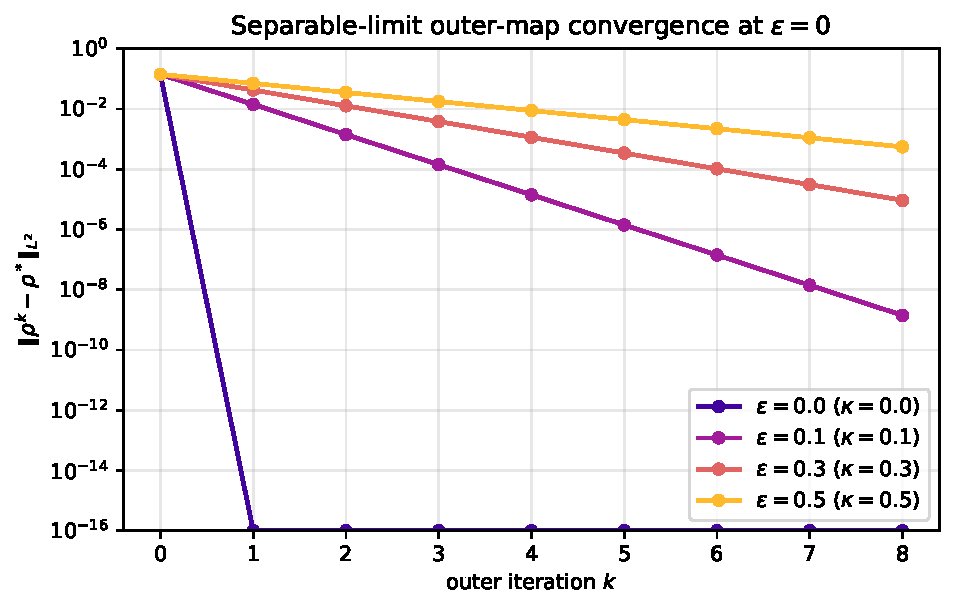
\includegraphics[width=.62\textwidth]{figures/exp1_analytic.pdf}
\caption{Separable-limit ablation.  At \(\eps=0\), the outer wrapper collapses
to one separable inner solve; for \(\eps>0\), the decay follows the predicted
geometric rate.}
\label{fig:separable_limit_neurips}
\end{figure}

\begin{table}[t]
\centering
\begin{tabular}{rrrr}
\toprule
\(\eps\) & theory \(\kappa\) & empirical \(\hat\kappa\) & final error \\
\midrule
0.10 & 0.100 & 0.100 & \(3.5{\times}10^{-14}\) \\
0.50 & 0.500 & 0.500 & \(8.6{\times}10^{-6}\) \\
0.90 & 0.900 & 0.900 & \(1.0{\times}10^{-2}\) \\
1.00 & 1.000 & 1.000 & \(3.5{\times}10^{-2}\) \\
1.30 & 1.300 & 1.300 & \(8.2{\times}10^{-1}\) \\
1.50 & 1.500 & 1.500 & \(4.6{\times}10^{0}\) \\
\bottomrule
\end{tabular}
\caption{Density-only linearized phase transition with \(\lambda=L_R=1\).}
\label{tab:phase_neurips}
\end{table}

\begin{figure}[t]
\centering
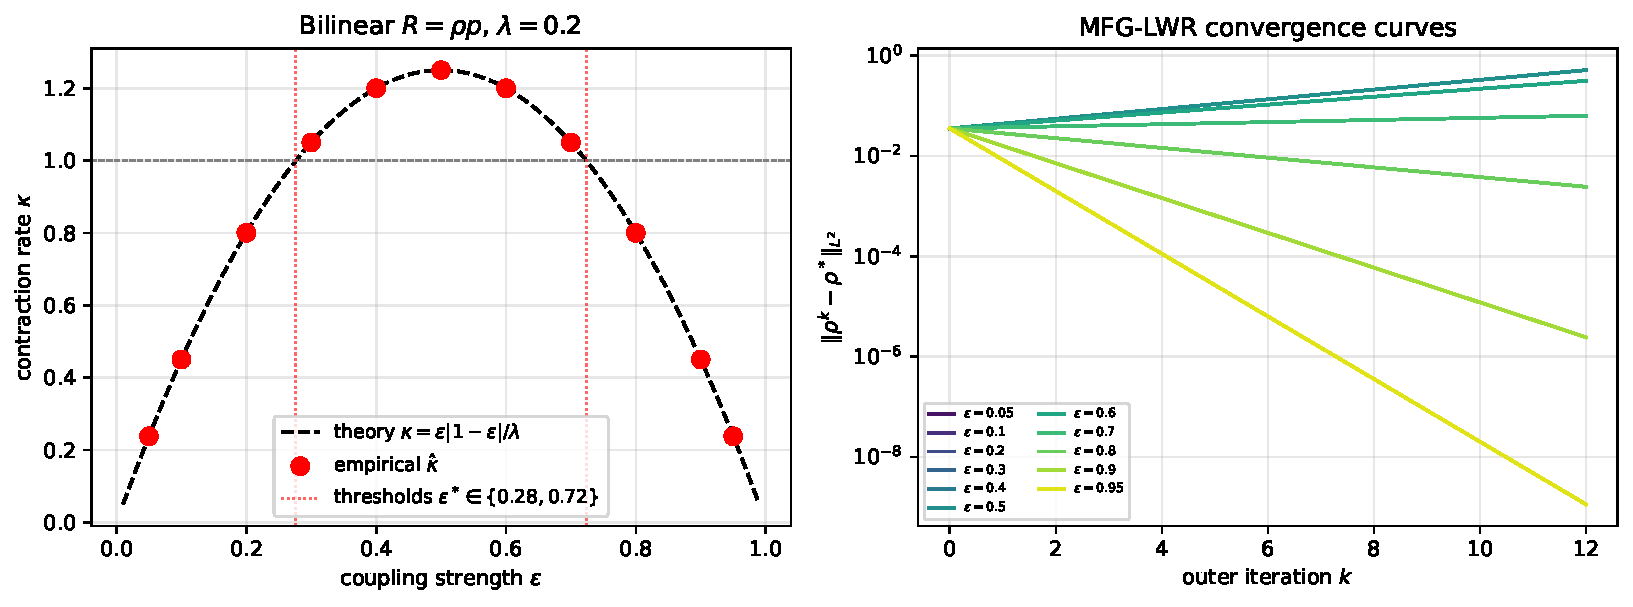
\includegraphics[width=.82\textwidth]{figures/exp2_traffic.pdf}
\caption{Traffic-flow sharpness experiment.  The bilinear density--momentum
coupling exhibits the predicted two-threshold behavior in
\(\eps |1-\eps|/\lambda\).}
\label{fig:traffic_sharpness_neurips}
\end{figure}

\begin{figure}[t]
\centering
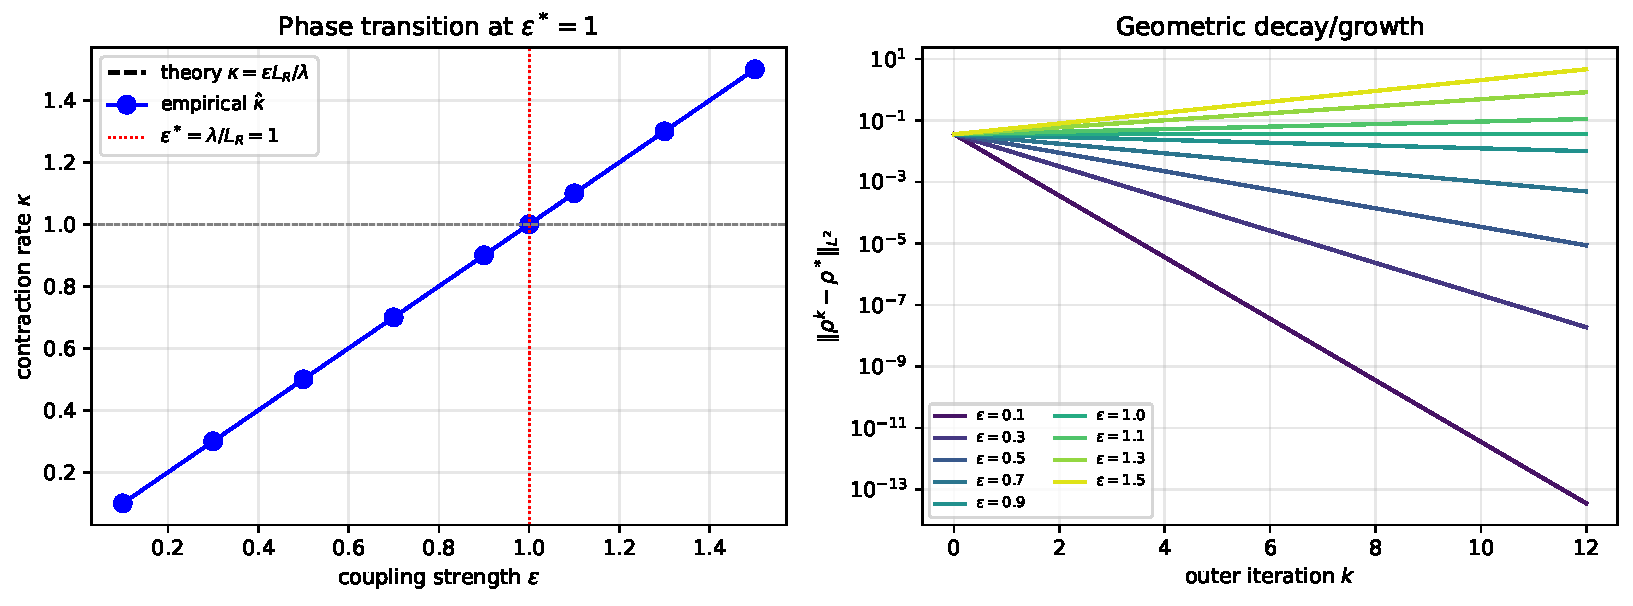
\includegraphics[width=.82\textwidth]{figures/exp3_phase_transition.pdf}
\caption{Density-only sharpness experiment.  The empirical contraction factor
matches the theory curve and transitions at \(\eps L_R/\lambda=1\).}
\label{fig:density_sharpness_neurips}
\end{figure}

These results are deliberately limited but diagnostic.  In all displayed cases,
the empirical contraction factor matches the theoretical factor to the reported
precision, including convergence below threshold, stagnation at threshold, and
growth above threshold.  The traffic experiment gives a motivating
non-separable example: for \(\lambda=0.2\), the predicted transition points are
\(\eps\approx0.276\) and \(\eps\approx0.724\), and the observed rates follow the
curve \(\eps |1-\eps|/\lambda\).

\section{Discussion and Limitations}

The result should be interpreted as a contraction theorem for the exact outer
map, not as a complete optimization guarantee for GAN training.  Its value is
that it identifies a regime in which non-separable MFGs can be reduced to a
sequence of separable, GAN-compatible subproblems with an explicit rate.  A full
neural APAC-Net-style implementation, finite-training optimization analysis,
and benchmarking against MFDGM, PINN/DGM residual solvers, and finite-difference
reference methods remain outside the present analysis.  Important limitations
are the non-vacuum condition, bounded momentum, exact inner solves in the main
theorem, and the restriction to weak residual coupling.

\bibliographystyle{abbrvnat}
\bibliography{references}

\appendix

\section{Stability Proof for \Cref{thm:l2_contraction_neurips}}

\begin{lemma}[Lasry--Lions stability identity]
\label{lem:ll_identity}
Let \((\varphi_i,\rho_i)\) solve the two frozen subproblems corresponding to
\(\bar\rho_i\), with the same initial density and terminal cost.  Write
\[
\delta\varphi=\varphi_1-\varphi_2,\quad
\delta\rho=\rho_1-\rho_2,\quad
\delta p=\nabla\varphi_1-\nabla\varphi_2.
\]
Then
\[
\lambda\norm{\delta\rho}_{L^2((0,T)\times\Omega)}^2
\leq \int_0^T A(t)\,dt ,
\]
where
\[
A(t)=\int_\Omega [H^1(x,p_1)-H^2(x,p_2)]\delta\rho\,dx
-\int_\Omega \delta p\cdot[
\rho_1\nabla_pH^1(x,p_1)-\rho_2\nabla_pH^2(x,p_2)]\,dx .
\]
\end{lemma}

\begin{proof}
Computing \(\frac{d}{dt}\int_\Omega \delta\varphi\,\delta\rho\,dx\), using the
HJB and FP equations, and integrating by parts gives
\[
\frac{d}{dt}\int_\Omega \delta\varphi\,\delta\rho\,dx
= A(t)-\int_\Omega (f_0(x,\rho_1)-f_0(x,\rho_2))\delta\rho\,dx .
\]
The boundary term vanishes after integration over \([0,T]\), because
\(\delta\rho(0,\cdot)=0\) and \(\delta\varphi(T,\cdot)=0\).  Strong
monotonicity of \(f_0\) therefore yields
the claim.
\end{proof}

\begin{lemma}[Frozen-Hamiltonian estimate]
\label{lem:frozen_estimate}
Under \Cref{ass:neurips}, the quantity \(A(t)\) in
\Cref{lem:ll_identity} satisfies
\[
  A(t)\leq
  \eps L_R\norm{\delta\bar\rho(t)}_{L^2(\Omega)}
       \norm{\delta\rho(t)}_{L^2(\Omega)}
  +B_\eps\norm{\delta\bar\rho(t)}_{L^2(\Omega)}^2 .
\]
\end{lemma}

\begin{proof}
Write \(H^i=H_0+\eps R^i\), where
\(R^i(x,p)=R(x,\bar\rho_i(x,t),p)\).  Split \(A=A_0+\eps A_R\).  For the
base Hamiltonian,
\[
A_0(t)=\int_\Omega [H_0(p_1)-H_0(p_2)]\delta\rho\,dx
-\int_\Omega \delta p\cdot[
\rho_1\nabla_pH_0(p_1)-\rho_2\nabla_pH_0(p_2)]\,dx .
\]
Using \(\delta\rho=\rho_1-\rho_2\), this can be rearranged as
\[
A_0(t)=
-\int_\Omega \rho_1\bigl[
H_0(p_2)-H_0(p_1)-\nabla_pH_0(p_1)\cdot(p_2-p_1)
\bigr]dx
-\int_\Omega \rho_2\bigl[
H_0(p_1)-H_0(p_2)-\nabla_pH_0(p_2)\cdot(p_1-p_2)
\bigr]dx .
\]
Strong convexity and \(\rho_i\geq\rho_{\min}\) give
\[
  A_0(t)\leq -c_0\rho_{\min}\int_\Omega |\delta p|^2\,dx .
\]
For the residual part, add and subtract \(R(x,\bar\rho_1,p_2)\) and
\(\nabla_pR(x,\bar\rho_1,p_2)\).  The terms involving
\(\bar\rho_1-\bar\rho_2\) are bounded by the Lipschitz assumption in density:
\[
|A_{R,\rho}(t)|
\leq L_R\norm{\delta\bar\rho(t)}_{L^2(\Omega)}
       \norm{\delta\rho(t)}_{L^2(\Omega)} .
\]
There is also a frozen-density contribution in the velocity field,
\(\nabla_pR(x,\bar\rho_1,p)-\nabla_pR(x,\bar\rho_2,p)\).  The
\(L_{p\rho}\)-Lipschitz assumption gives
\[
  \eps\left|\int_\Omega
  \rho_2\,\delta p\cdot
  [\nabla_pR(x,\bar\rho_1,p_2)-\nabla_pR(x,\bar\rho_2,p_2)]\,dx\right|
  \leq
  \eps L_{p\rho}\rho_{\max}
  \norm{\delta p}_{L^2}\norm{\delta\bar\rho}_{L^2}.
\]
The remaining residual terms depend only on the momentum difference.  Taylor's
formula and \(|\nabla_pR|+|\nabla_{pp}^2R|\leq L_{R,p}\), together with
\(\rho_i\leq\rho_{\max}\), yield the conservative bound
\[
|A_{R,p}(t)|\leq 3L_{R,p}\rho_{\max}
\int_\Omega |\delta p|^2\,dx .
\]
Combining this with the negative base contribution gives
\[
  -\alpha_\eps\norm{\delta p}_{L^2}^2
  +\eps L_{p\rho}\rho_{\max}
  \norm{\delta p}_{L^2}\norm{\delta\bar\rho}_{L^2}.
\]
Maximizing the right-hand side over \(\norm{\delta p}_{L^2}\) gives
\[
  B_\eps\norm{\delta\bar\rho}_{L^2}^2,\qquad
  B_\eps=\frac{\eps^2L_{p\rho}^2\rho_{\max}^2}{4\alpha_\eps}.
\]
Together with the density-variation term this proves the estimate.
\end{proof}

\begin{proof}[Proof of \Cref{thm:l2_contraction_neurips}]
\Cref{lem:ll_identity,lem:frozen_estimate} give
\[
\lambda\norm{\delta\rho}_{L^2}^2
\leq \eps L_R\norm{\delta\bar\rho}_{L^2}\norm{\delta\rho}_{L^2}
+B_\eps\norm{\delta\bar\rho}_{L^2}^2 .
\]
If \(\delta\bar\rho\neq0\), divide by
\(\norm{\delta\bar\rho}_{L^2}^2\) and solve the resulting quadratic inequality
for \(\norm{\delta\rho}_{L^2}/\norm{\delta\bar\rho}_{L^2}\), obtaining
\(\kappa_\eps\).  The case \(\delta\bar\rho=0\) is trivial.  Banach's
fixed-point theorem gives existence and uniqueness of the outer fixed point and
the geometric convergence bound.
\end{proof}

\section{Perturbed Inner Solves}

If the inner solver returns \(\rho_N^{k+1}\) with
\(\norm{\rho_N^{k+1}-\mathcal{T}(\rho_N^k)}_{L^2}\leq\delta_N\), then
\[
  \norm{\rho_N^k-\rho^\star}_{L^2}
  \leq
  \kappa_\eps^k\norm{\rho^0-\rho^\star}_{L^2}
  +\frac{\delta_N}{1-\kappa_\eps}.
\]
This follows by iterating
\(\norm{\rho_N^{k+1}-\rho^\star}_{L^2}\leq
\delta_N+\kappa_\eps\norm{\rho_N^k-\rho^\star}_{L^2}\).

\section{Reproducibility Details}

All experiments in the paper are deterministic linearized-map evaluations and
use no external datasets.  The scripts are included in the supplementary code
and can be run with Python, NumPy, and Matplotlib:
\begin{verbatim}
python3 code/experiments/exp1_analytic.py
python3 code/experiments/exp2_traffic.py
python3 code/experiments/exp3_phase_transition.py
\end{verbatim}
Each script prints the table values and regenerates the corresponding PDF
figure.  A GPU is not required.

\newpage
\input{checklist.tex}

\end{document}
